\documentclass{article}
    % General document formatting
    \usepackage[margin=0.7in]{geometry}
    \usepackage[parfill]{parskip}
    \usepackage[utf8]{inputenc}
    \usepackage{amsmath}
    \usepackage{amssymb}
    \usepackage{tikz}
    \usepackage{fancyhdr}
    \usepackage{listings}

\pagestyle{fancy}
\fancyhf{}
\rhead{Edgar Jacob Rivera Rios - A01184125}

\begin{document}
\begin{titlepage}

    \newcommand{\HRule}{\rule{\linewidth}{0.5mm}} % Defines a new command for the horizontal lines, change thickness here

    \center % Center everything on the page

    %----------------------------------------------------------------------------------------
    %	HEADING SECTIONS
    %----------------------------------------------------------------------------------------

    \textsc{\LARGE Tecnológico de Monterrey}\\[1.5cm] % Name of your university/college
    \textsc{\Large Fundamentos de computación}\\[0.5cm] % Major heading such as course name
    %\textsc{\large Minor Heading}\\[0.5cm] % Minor heading such as course title

    %----------------------------------------------------------------------------------------
    %	TITLE SECTION
    %----------------------------------------------------------------------------------------

    \HRule \\[0.4cm]
    { \huge \bfseries Homework 2}\\[0.4cm] % Title of your document
    \HRule \\[1.5cm]

    %----------------------------------------------------------------------------------------
    %	AUTHOR SECTION
    %----------------------------------------------------------------------------------------

    \begin{minipage}{0.4\textwidth}
    \begin{flushleft} \large
    \emph{Student:}\\
    Jacob \textsc{Rivera} % Your name
    \end{flushleft}
    \end{minipage}
    ~
    \begin{minipage}{0.4\textwidth}
    \begin{flushright} \large
    \emph{Professor:} \\
    Dr. Hugo \textsc{Terashima} % Supervisor's Name
    \end{flushright}
    \end{minipage}\\[2cm]

    % If you don't want a supervisor, uncomment the two lines below and remove the section above
    %\Large \emph{Author:}\\
    %John \textsc{Smith}\\[3cm] % Your name

    %----------------------------------------------------------------------------------------
    %	DATE SECTION
    %----------------------------------------------------------------------------------------

    {\large \today}\\[2cm] % Date, change the \today to a set date if you want to be precise

    %----------------------------------------------------------------------------------------
    %	LOGO SECTION
    %----------------------------------------------------------------------------------------

    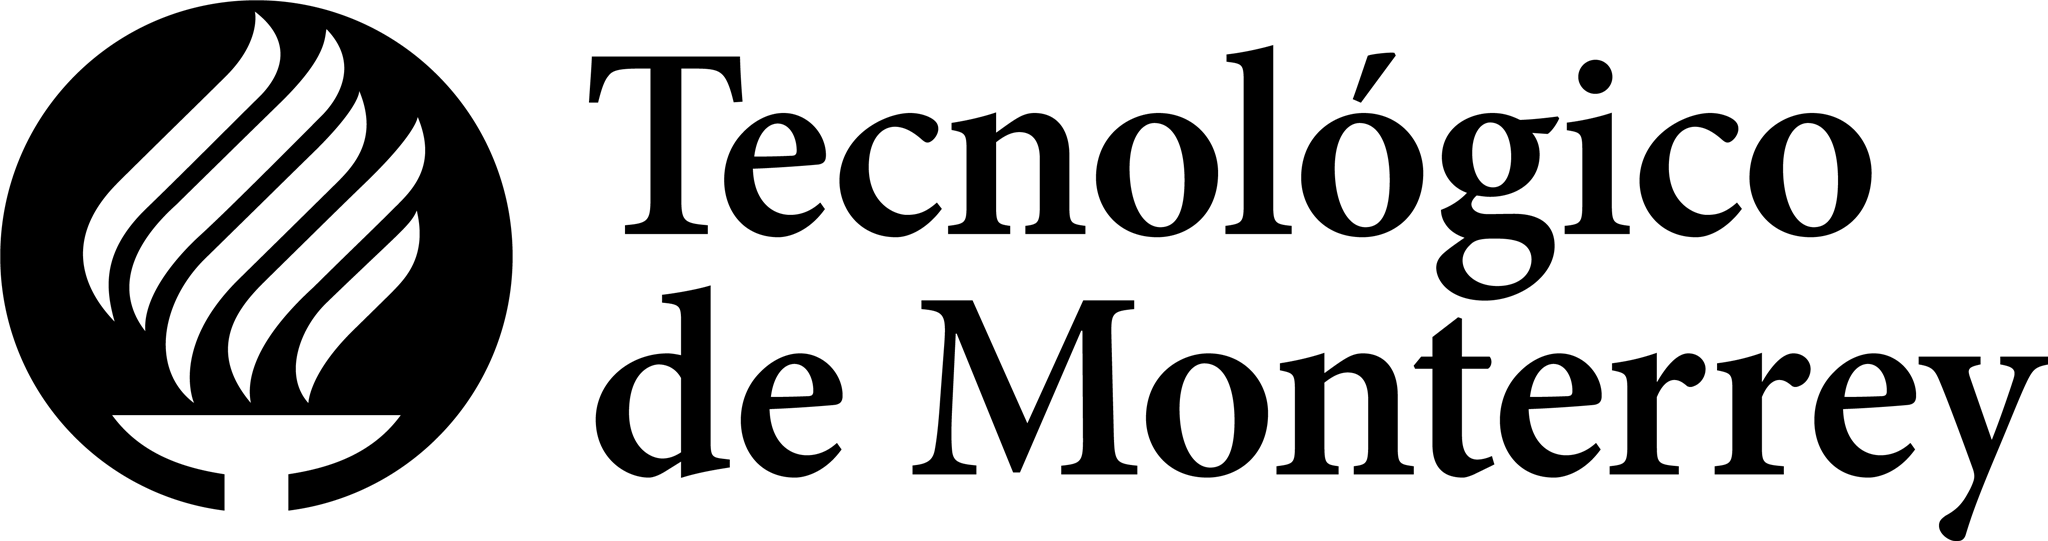
\includegraphics[width=0.4\textwidth,height=\textheight,keepaspectratio]{logo-tec-negro.png} % Include a department/university logo - this will require the graphicx package

    %----------------------------------------------------------------------------------------

    \vfill % Fill the rest of the page with whitespace

\end{titlepage}


\section{Problems}
Solve the following problems:
\begin{enumerate}
    \item Use  the  substitution  method  to  solve  the  following  recurrences  and  determine  their  corresponding complexity. Establish the proper initial conditions for each problem.
    \begin{enumerate}
        \item $T(n) = 4T(n/2) +n^4$
        \begin{equation*}
            T(n)=\begin{cases}
              b & \text{if $n = 1$}.\\
              aT(\frac{n}{c}) + bn^x, & \text{otherwise}.
            \end{cases}
        \end{equation*}
        \begin{equation*}
            n = 2^k
        \end{equation*}

        \begin{align*}
            T(n) &= 2^2T(n/2) + n^4\\
            &= 2^2(2^2T(\frac{n}{2^2}) + (\frac{n}{2})^4) + n^4\\
            &= 2^4(2^2T(\frac{n}{2^3}) + (\frac{n}{2^2})^4 )+ \frac{n^4}{2^2} + n^4\\
            &= 2^6(2^2T(\frac{n}{2^4}) + (\frac{n}{2^3})^4)+ \frac{n^4}{2^4} + \frac{n^4}{2^2} + n^4\\
            &= 2^8T(\frac{n}{2^4}) + \frac{n^4}{2^6}+ \frac{n^4}{2^4} + \frac{n^4}{2^2} + n^4\\
            &=2^{2k}T(\frac{n}{2^k}) +\sum^{k -1}_{i=0} \frac{n^4}{2^{2i}}\\
            &=2^{2k}T(\frac{n}{2^k}) +n^4 \sum^{k -1}_{i=0} \frac{1}{2^{2i}}\\
            &=2^{n}T(0) +n^4 \sum^{k -1}_{i=0} \frac{1}{2^{2i}}\\
            &=n^4 \sum^{k -1}_{i=0} \frac{1}{2^{2i}}\\
            &=n^4 \sum^{k -1}_{i=0} 2^{-2i}\\
            &=n^4 * \frac{1-2^k}{1-2}\\
            &=n^4\\
            &\in O(n^4)
        \end{align*}

        \item $T(n) = 3T(n/3) + n log(n)$
        \begin{equation*}
            n = 3^k
        \end{equation*}
        \begin{align*}
            T(n) &= 3T(n/3) + n log(n)\\
            &= 3(3T(\frac{n}{3^2}) + \frac{n}{3} log(\frac{n}{3})) + n log(n)\\
            &= 3^k T(\frac{n}{3^k}) + \sum_{i =0 }^{k-1} n log(\frac{n}{3^i})\\
            &= 3^k T(0) + \sum_{i =0 }^{k-1}n log(\frac{n}{3^i})\\
            &= n \sum_{i =0 }^{k-1} log(\frac{n}{3^i})\\
            &= n log^2(n) \\
            &\in n log^2(n)
        \end{align*}

        \item $T(n) = 3T(n/3) + \frac{\sqrt{n}}{log(n)}$
        \begin{equation*}
            n = 3^k
        \end{equation*}
        \begin{align*}
            T(n) &= 3T(n/3) + \frac{\sqrt{n}}{log(n)}\\
            &= 3(3T(\frac{n}{3^2}) + \frac{\sqrt{n/3}}{log(n/3)}) + \frac{\sqrt{n}}{log(n)}\\
            &= 3^2T(\frac{n}{3^2}) + 3\frac{\sqrt{n/3}}{log(n/3)}) + \frac{\sqrt{n}}{log(n)}\\
            &= 3^2(3T(\frac{n}{3^3}) + \frac{\sqrt{n/3}}{log(n/3)}) + 3\frac{\sqrt{n/3}}{log(n/3)} + \frac{\sqrt{n}}{log(n)}\\
            &= 3^3T(\frac{n}{3^3}) + 3^2\frac{\sqrt{n/3}}{log(n/3)} + 3\frac{\sqrt{n/3}}{log(n/3)} + \frac{\sqrt{n}}{log(n)}\\
            &= 3^kT(\frac{n}{3^k}) + \sum_{i =0}^{k-1}3^i\frac{\sqrt{n/3^i}}{log(n/3^i)} \\
            &= 3^kT(0) + \sum_{i =0}^{k-1}3^i\frac{\sqrt{n/3^i}}{log(n/3^i)}\\
            &= \sum_{i =0}^{k-1}3^i\frac{\sqrt{n/3^i}}{log(n/3^i)}\\
            &= \sum_{i =0}^{k-1}3^i\frac{\sqrt{n/3^i}}{log(n/3^i)} \leq 3^{log(n)}\\
            \in O(3^{log(n)})
        \end{align*}
        \item $T(n) = T(n - 3) +n$
        \begin{equation*}
            n = 3k
        \end{equation*}
        \begin{align*}
            T(n) &= T(n -3) + n\\
            T(n-1) &= T(n-4) + n\\
            T(n-3) &= T(n-6) + n\\
            &= T(n-6) + 2n\\
            &= T(n-3k) + kn\\
            &= T(n-3\frac{n}{3}) + \frac{n}{3}n\\
            &= T(0) + \frac{n}{3}n\\
            &= \frac{n^2}{3}\\
            &\in O(n^2)
        \end{align*}
    \end{enumerate}
    \item  Modify the algorithm for multiplying two numbers $X$ and $Y$(that with complexity $n^{1,59}$), dividing each number in three parts. Describe the algorithm and derive its complexity. Is it better than dividing by two parts? Explain.

    The algorithm would keep the same functioning as the old one, the only difference being how it's divided. As such, the recurrence would be

    \begin{align*}
        T(n) = 8T(n/3) + kn
    \end{align*}

    Which results in a complexity $O(n^{1.893})$ which would result in worst performance than using a two parts split

    \item The run time of an algorithm $A$ for solving a problem is given by the recurrence $T(n) = 7T(n/4) + n.$ A different algorithm $A^{\prime}$ for solving the same problem has a running time given by $T^{\prime}(n) =aT^{\prime}(n/7) +n$. Determine  the  integer  value $a$ with  which  algorithm $A$ is  better  than  algorithm $A^{\prime}$.  Explain  your process.

    By the use of the master theorem, we know that $T(n) \in O(n^{1.404})$ and $T'(n) \in O(n)$, so only when $n = 1$ the algorithms are going to make the same number of steps.

    \item For each of the following algorithms, which each receive an integer as input, determine what they do,establish the corresponding recurrence,and solve it to find the computational complexity.
    \begin{lstlisting}
    ALGORITHM BR(n)
        // Input a positive integer n
        if n = 1 return 1
        else return BR(floor(n/2)) + 1
    \end{lstlisting}

    This algorithm returns the power of 2 closest to the input number, without surpassing it. The recurrence would be: $T(n) = T(n/2) + 1$, which complexity would be $O(log(n))$

    \begin{lstlisting}
    ALGORITHM Question(n)
        // Input a positive integer n
        if n = 1 return 1
        else return Question(n-1) + n*n*n
    \end{lstlisting}

    This algorithm gives us the sum of the cubes of all numbers until n. As such, the recurrence would be $T(n) = T(n - 1) + n^3$, which results in complexity of $O(n^4)$
    \begin{align*}
        n = k
        T(n) &= T(n - 1) + n^3\\
        T(n - 1 ) &= T(n - 2) + 2n^3\\
        T(n) &= T(n - k) + kn^3\\
        T(n) &= T(0) + n^4\\
        \in O(n^4)
    \end{align*}

    \item The Towers of Hanoi problem is often used as an example when teaching recursion. Six disks of different sizes are piled on a peg in order by size, with the largest at the bottom. There are two empty pegs. The problem is to move all the disks to the third peg by moving only one at a time a never placing a disk on top of a smaller one. The second peg may be used for intermediate moves. The usual solution recursively moves all but the last disk from the starting peg to the spare peg, then moves the remaining disks on the start peg to the destination peg, and then recursively moves all the others from the spare peg to the destination peg. Illustrate these steps and explain the procedure in a pseudocode. Write a recurrence equation to determine the number of moves done and solve it.

    The solution proposed would be fairly easy to implement following the next pseudocode:
    \begin{lstlisting}
    Towers(disk, source, destination, auxiliar)
        //Disk is the number of the disk to be moved, source is the starting
        point, destination is the goal and auxiliar is the spare peg
        if (disk == 1)
            move(disk, destination)
        else
            Towers(n - 1, source, auxiliar, destination)
            move(disk, destination)
            Towers(n - 1, auxiliar, destination, source)
    \end{lstlisting}

    \begin{align*}
        T(1) &= 1\\
        n &= k +1\\
        T(n) &= 2T(n-1)\\
        &= 2^2T(n-2)\\
        &= 2^kT(n-k)\\
        &= 2^{n-1}T(n-(n -1))\\
        &= 2^{n-1}T(1)\\
        &= 2^{n-1}\\
        &\in \theta(2^{n-1})
    \end{align*}

\end{enumerate}
\end{document}